\documentclass[11pt]{beamer}

\input{BeamerSettings}

\definecolor{codegreen}{rgb}{0,0.6,0}
\definecolor{codegray}{rgb}{0.5,0.5,0.5}
\definecolor{codepurple}{rgb}{0.58,0,0.82}
\definecolor{backcolour}{rgb}{0.95,0.95,0.92}

\lstdefinestyle{mystyle}{
    backgroundcolor=\color{backcolour},
    commentstyle=\color{codegreen},
    keywordstyle=\color{magenta},
    numberstyle=\tiny\color{codegray},
    stringstyle=\color{codepurple},
    basicstyle=\ttfamily\tiny,
    breakatwhitespace=false,
    breaklines=true,
    captionpos=b,
    keepspaces=true,
    numbers=left,
    numbersep=5pt,
    showspaces=false,
    showstringspaces=false,
    showtabs=false,
    tabsize=2,
    xleftmargin=0.05\textwidth,
    xrightmargin=0.45\textwidth
}

\newcommand{\inlinecode}[1]{\colorbox{backcolour}{\lstinline{#1}}}

\lstset{style=mystyle}

\author{\textbf{Zachery~Crandall}}
\title[VSCode~Setup]{Setting~Up~Visual~Studio~Code~(VSCode)}
\institute[Ames]{
    Scientist I\\
    Ames National Laboratory\linebreak

    PhD in Physical Chemistry\\
    MS in Computer Science and Robotics\\
} 

\date[2026-06-02]{2026 SIMCODES Bootcamp}

\begin{document}

\TitleSlide

\TwoRowSlide{
    What is an IDE?
} {
    \BulletList{
        \item IDE == Integrated development environment
    }

    \AddPicture{fig/notepad_hello_world.png}
}{\AddPicture{fig/vscode_hello_world.png}}{}

\ContentSlide{
    Installing VSCode
} {
    \BulletList{
        \item Go to \text{https://code.visualstudio.com}
        \item Click ``Download for Your\_OS''
        \item Open the installer
    }

    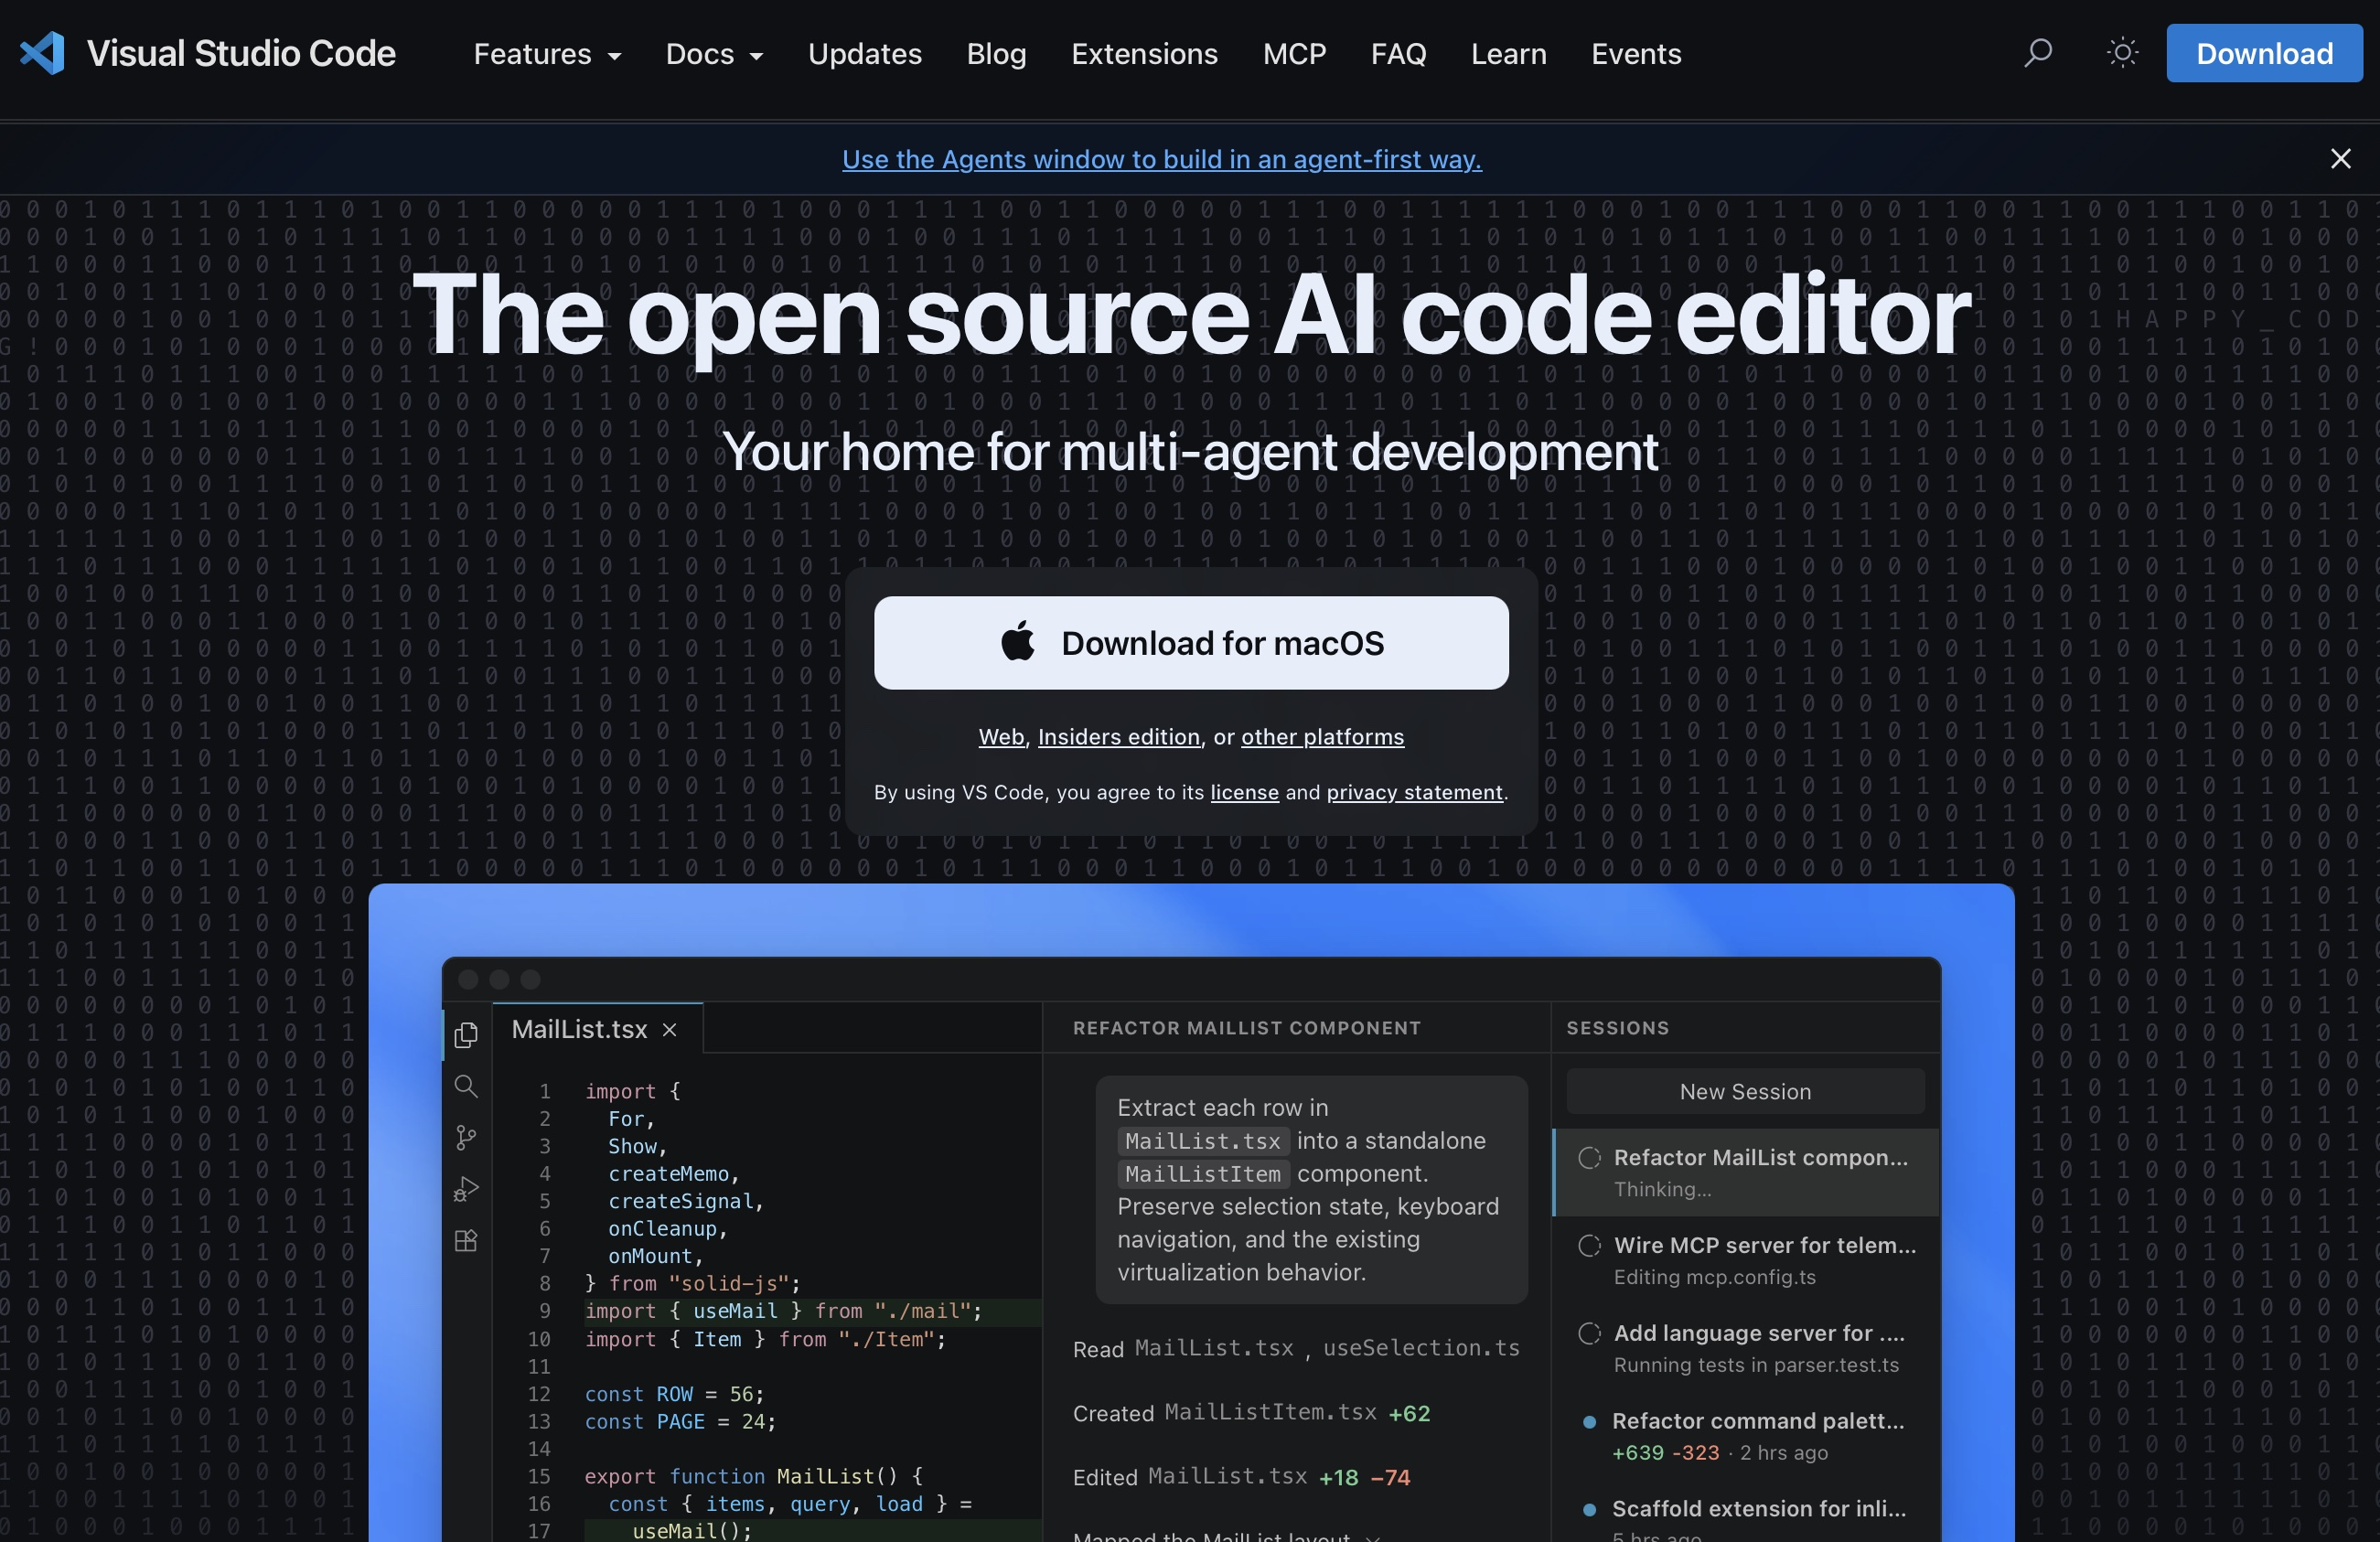
\includegraphics[height=0.66\textheight,keepaspectratio]{fig/macos_download.jpg}
}{}


\TwoColumnSlide{Installing VSCode}
{
    Windows
    \BulletList{
        \item Make sure all ``Open with Code'' options are checked
        \item Finish and launch VSCode
    }
    \begin{center}
    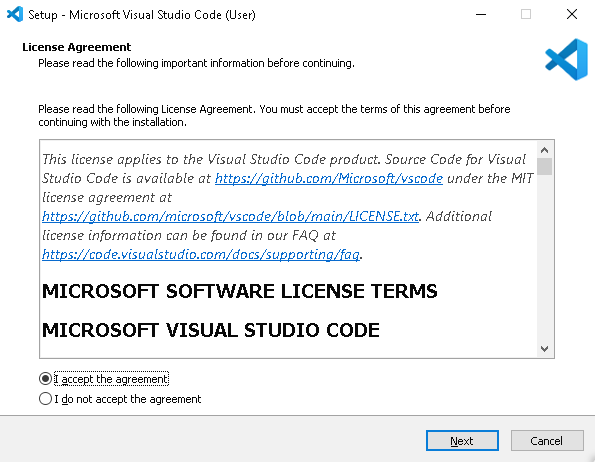
\includegraphics[width=0.62\textwidth,keepaspectratio]{fig/vscode_windows_accept_license.png}
    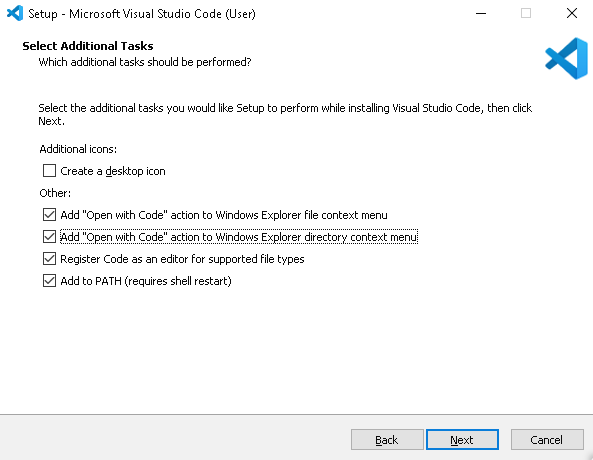
\includegraphics[width=0.62\textwidth,keepaspectratio]{fig/vscode_windows_additional_tasks.png}
    \end{center}
}
{
    MacOS
    \BulletList{
        \item Drag icon to ``Applications''
        \item Open ``Visual Studio Code'' from Launchpad
    }
    \begin{center}
    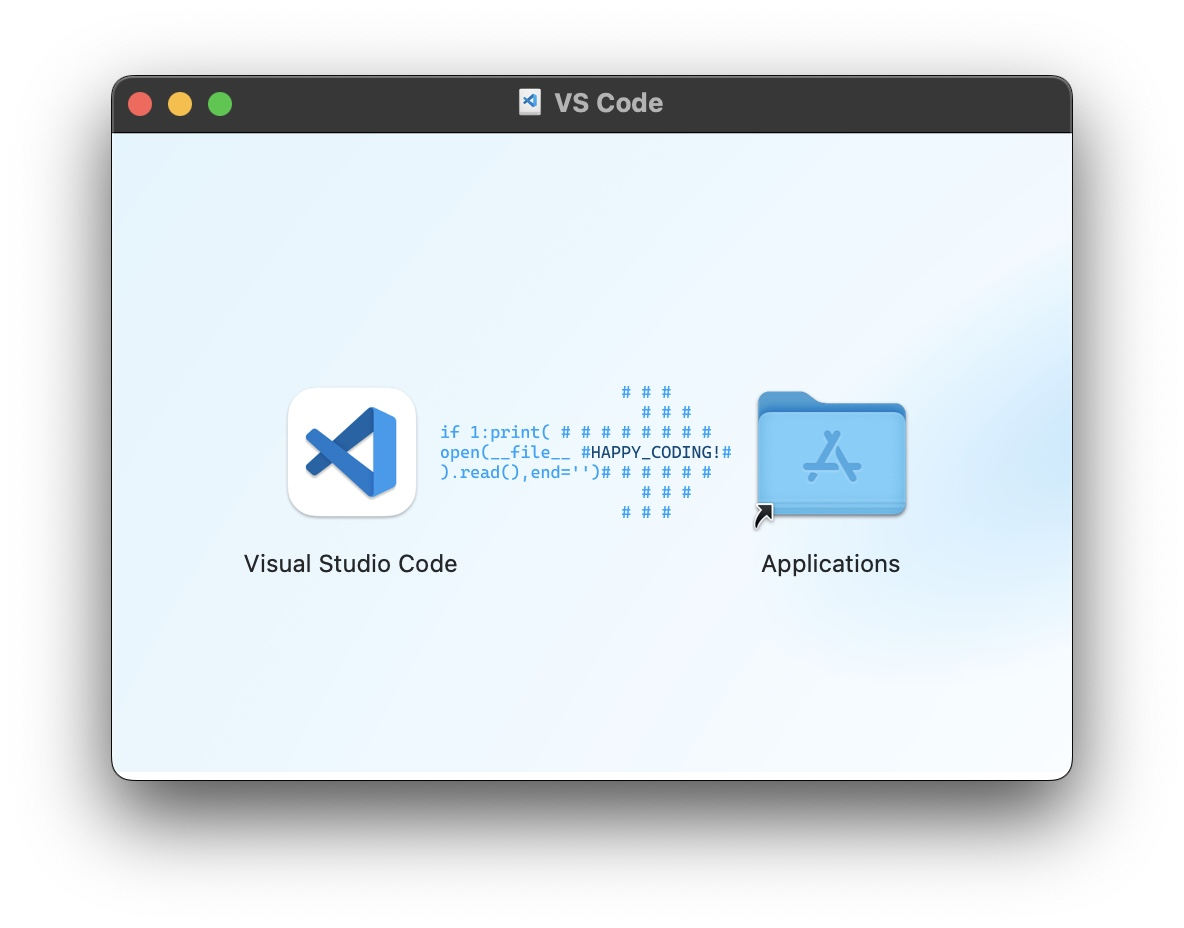
\includegraphics[width=0.55\textwidth,keepaspectratio]{fig/macos_install.jpg}
    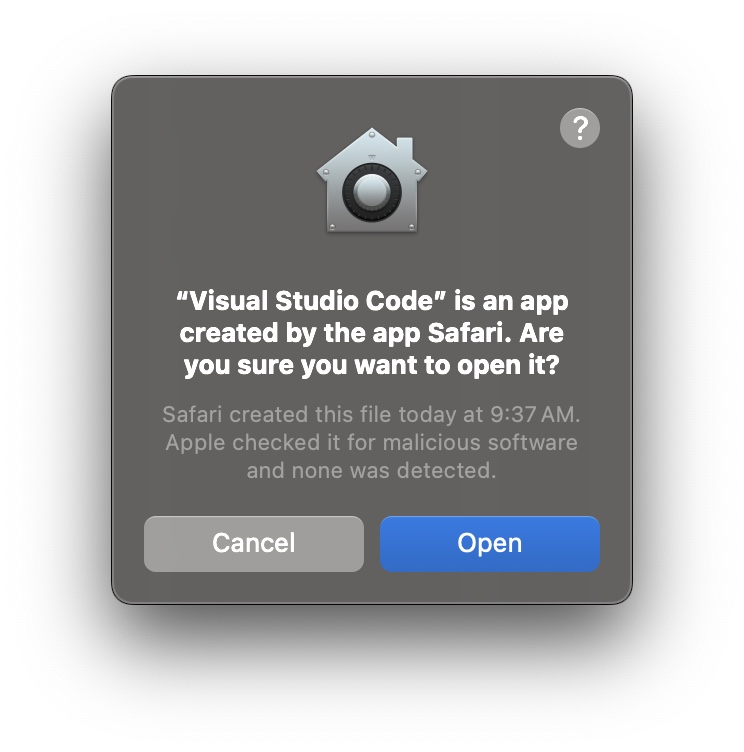
\includegraphics[width=0.55\textwidth,keepaspectratio]{fig/macos_allow.jpg}
    \end{center}
}
{}

\ContentSlide{Notes on AI/Agents}
{
    \BulletList{
        \item VSCode may prompt you to sign in to gain access to AI models/agents.
        \item Do so at your own risk.
        \item You are responsible for every line of code you commit to a repository.
        \item If you let AI develop for you, you must validate the results.
        \item Validation is nearly impossible unless you are experienced already.
    }
}
{}

\ContentSlide{
    Installing Python (Windows)
}{
    \BulletList{
        \item Go to \text{https://python.org/downloads/}
        \item Click ``Download Python install manager''
        \item Open the installer
    }

    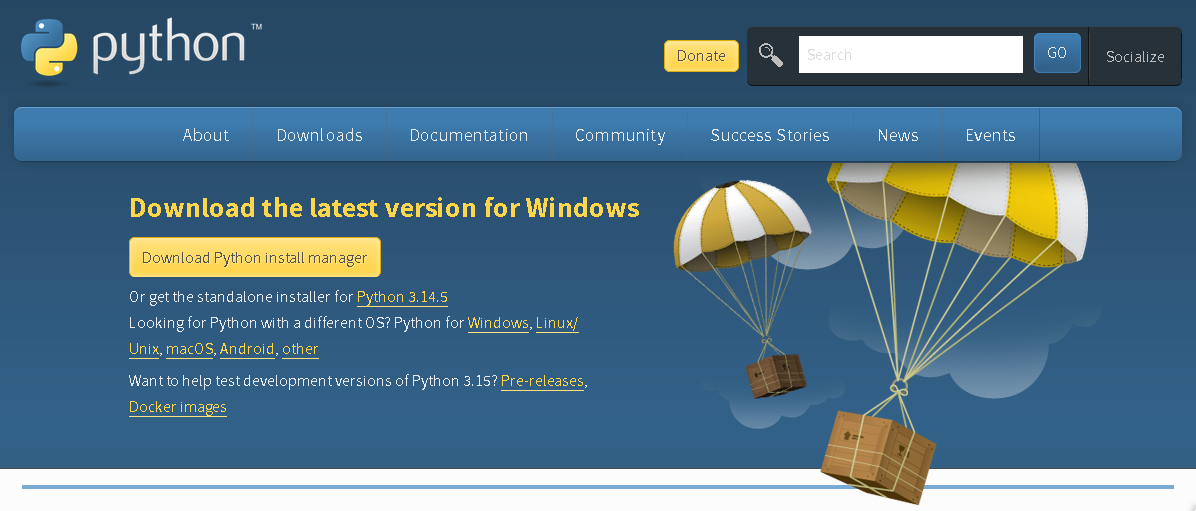
\includegraphics[width=1.1\textwidth,keepaspectratio]{fig/python_windows_website_install_manager.png}
}{}

\ContentSlide{
    Installing Python (Windows)
}{
    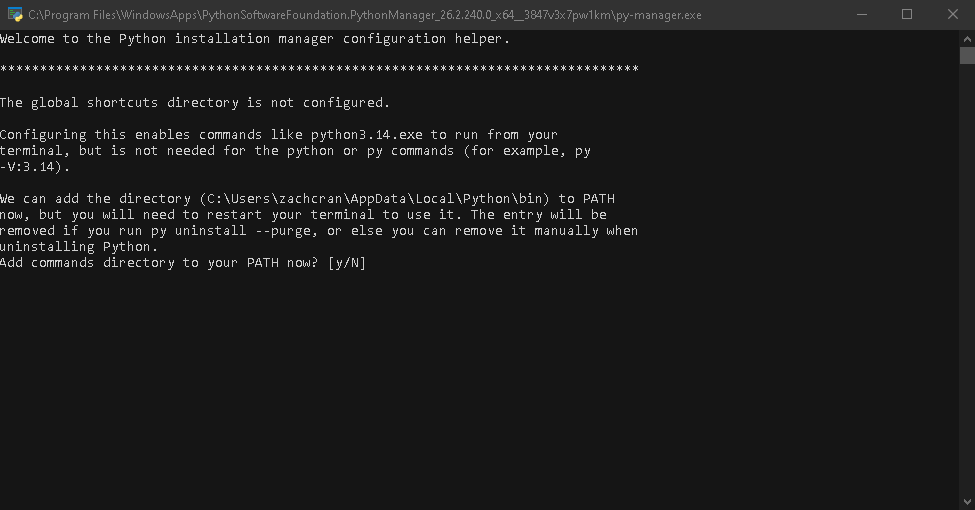
\includegraphics[width=1.0\textwidth,keepaspectratio]{fig/windows_install_manager_add_to_path.png}
}{}

\ContentSlide{
    Installing Python (Windows)
}{
    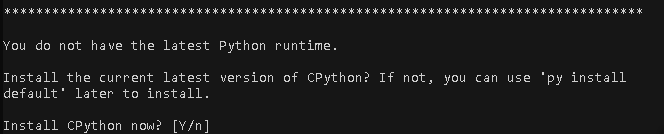
\includegraphics[width=1.0\textwidth,keepaspectratio]{fig/windows_install_manager_install_latest_version.png}
}{}

\ContentSlide{
    Testing your Python Install
}{
    \BulletList{
        \item Open VSCode
        \item At the top, select ``Terminal'', ``New Terminal''
        \item Test the \textbf{interpreter}: Type ``python'' and press [Enter]
    }

    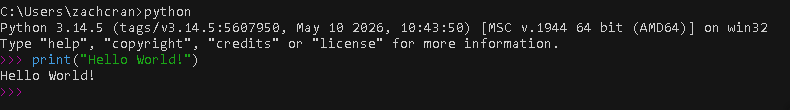
\includegraphics[width=1.1\textwidth,keepaspectratio]{fig/python_interpreter_hello_world.png}

    \BulletList{
        \item Note: The interpreter is a place to quickly test individual functions and small scripts, but you should not develop code here!!!
    }
}{}

\TwoColumnSlide{Installing Extensions}
{
    \BulletList{
        \item Search for ``Python'' in the extensions tab
        \item Install Python extensions (left)
        \item Install recommended extensions (right)
    }
}
{
    \begin{center}
    
\includegraphics[height=0.10\textheight,keepaspectratio]{fig/vscode_extensions_symbol.png}

    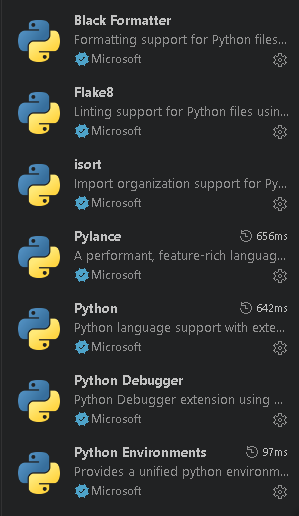
\includegraphics[height=0.50\textheight,keepaspectratio]{fig/vscode_extensions_python.png}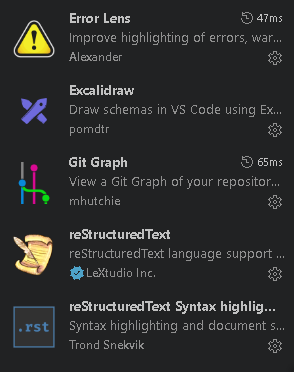
\includegraphics[height=0.50\textheight,keepaspectratio]{fig/vscode_extensions_other.png}
    \end{center}
}
{}

\ContentSlide{
    Testing your Development Environment
}{
    \BulletList{
        \item Make a new folder named ``hello\_world''
        \item Open VSCode in that folder
        \item In VSCode, make a new file called ``hello.py''
    }

    \begin{center}
    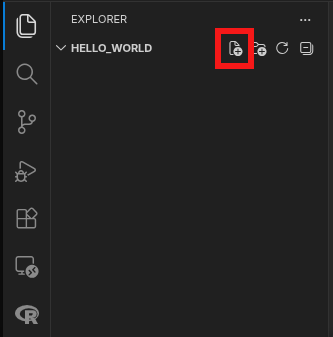
\includegraphics[width=0.6\textwidth,keepaspectratio]{fig/vscode_new_folder_button.png}
    \end{center}
}{}

\ContentSlide{
    Testing your Development Environment
}{
    \BulletList{
        \item Create and run the following code for a ``Hello World'' script
    }

    \begin{center}
    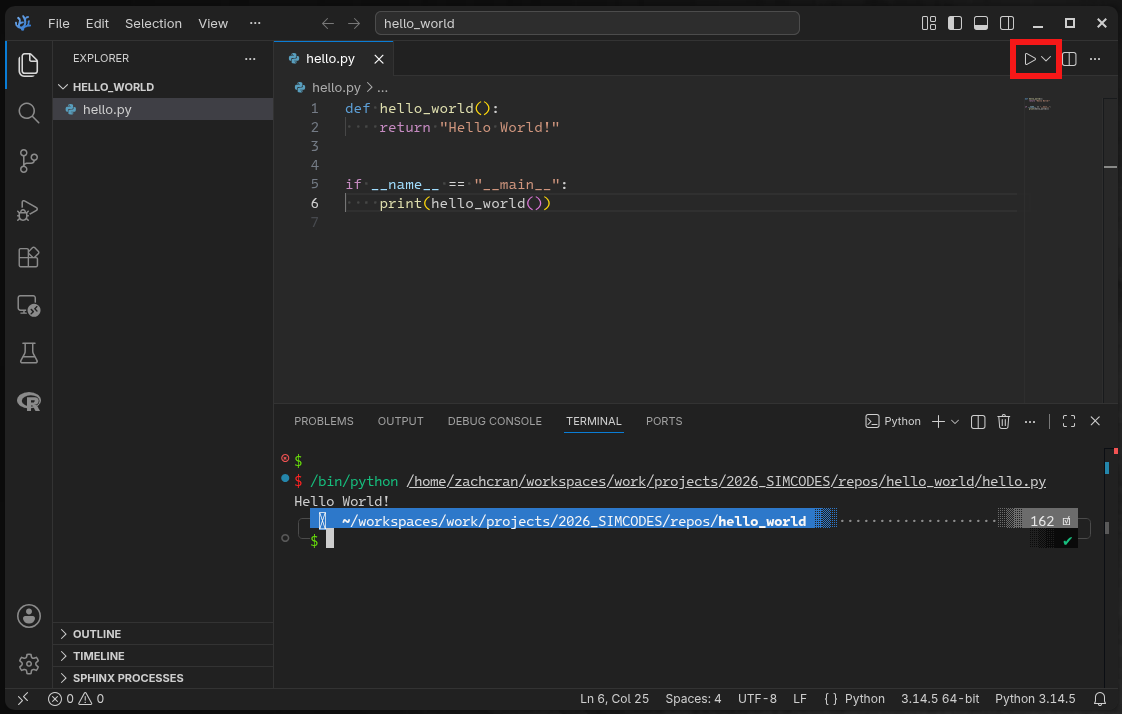
\includegraphics[width=1.0\textwidth,keepaspectratio]{fig/vscode_hello_world_script.png}
    \end{center}
}{}

\TwoColumnSlide{Acknowledgements}
{\BulletList{
    \item NSF for funding the REU.
    \item ISU and Ames National Lab
}}
{
    \AddPicture{fig/nsf.jpg}
}
{}

\BackupBegin{}

\ContentSlide{
    Installing Python (macOS)
}{
    \BulletList{
        \item Open VSCode
        \item At the top, select ``Terminal'', ``New Terminal''
        \item Install UV with the following command: \\curl -LsSf https://astral.sh/uv/install.sh $|$ sh
        \item Install Python: \\uv python install 3.14
    }
    \BulletList{
        \item Windows can also install UV at this point with:\\pip install -{}-user uv
    }
}{}

\ContentSlide{
    General Editor Settings
}{
    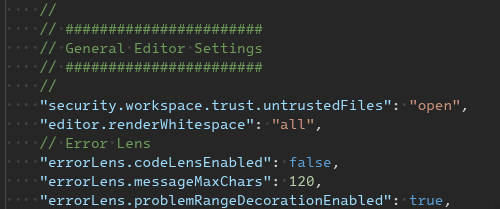
\includegraphics[width=1.0\textwidth,keepaspectratio]{fig/bonus_vscode_settings_editor_settings.png}
}{}

\ContentSlide{
    Python Settings
}{
    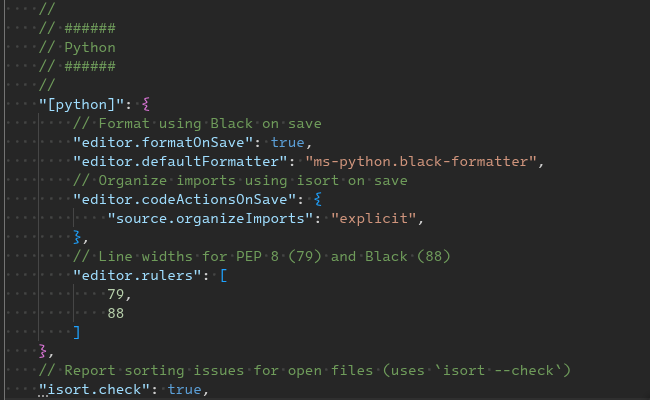
\includegraphics[width=1.0\textwidth,keepaspectratio]{fig/bonus_vscode_settings_python.png}
}{}

\ContentSlide{
    Telemetry Settings
}{
    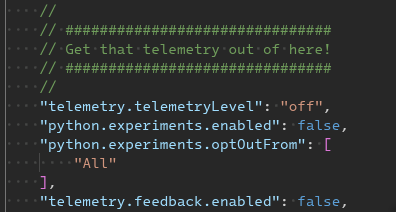
\includegraphics[width=1.0\textwidth,keepaspectratio]{fig/bonus_vscode_settings_telemetry.png}
}{}

\BackupEnd{}

\end{document}
